\hyphenation{
JSetL
Java
IntLVar
SetLVar
Constraint
JUnit
TCK
}

\chapter{Implementazione: Rappresentazione della Soluzione}\label{capImpl2}
In questo capitolo verranno descritte le classi Java implementate per la
specifica JSR-331 nell'ambito della risoluzione di un problema (CSP).

Per ogni classe descritta verrà introdotta l'interfaccia fornita dalla 
specifica e quindi, con maggior dettaglio, l'implementazione che riguarda
il solver JSetL.


\subsubsection{Risoluzione del problema}
Per rappresentare la risoluzione di un qualsiasi problema, la specifica JSR-331
utilizza le seguenti interfacce: 
\begin{itemize}
\item[-]\files{Solver};
\item[-]\files{SearchStrategy};
\item[-]\files{Solution};
\item[-]\files{SolutionIterator}.
\end{itemize}
Nelle prossime sezioni verranno descritte le suddette classi (implementazioni)
con i principali metodi.


%\section{Risoluzione del problema}
\section{Interfaccia \texttt{Solver}}\label{solver}
Per rappresentare la parte di risoluzione di un qualsiasi CSP, la specifica
JSR-331 utilizza l'interfaccia \files{Solver}. Il solver permette ad un utente
di risolvere un problema cercando una soluzione soddisfacibile od ottimale. Ecco
un esempio:
\begin{lstlisting}[language = Java,
                   caption = {una risoluzione di \files{problem}.}]
        problem.log("=== Find One solution:");
        Solver solver = problem.getSolver();
        Solution solution = solver.findSolution();
        if (solution != null)
          solution.log();
        else
          problem.log("No Solutions");
\end{lstlisting}
In questo semplice esempio il solver cerca una soluzione 
utilizzando una strategia di ricerca di default. La specifica definisce anche 
un'interfaccia per la strategia di ricerca come si vedrà nella sezione
\ref{search}.

\subsection{Come ottenere le soluzioni}
Lo scopo principale dell'interfaccia \files{Solver} è quello di dare all'utente
gli strumenti, dato un problema, per trovarne le soluzioni. Vengono quindi 
forniti i seguenti metodi:
\begin{lstlisting}[language = Java,
                   frame = single]
public Solution findSolution();
public Solution findSolution(ProblemState restoreOrNot);
public Solution findOptimalSolution(Objective objective, Var objectiveVar);
public Solution findOptimalSolution(Var objectiveVar);
public Solution[] findAllSolutions();
\end{lstlisting}
I primi due metodi cercano una soluzione del problema, utilizzano la strategia
di default o l'ultima strategia definita. Restituiscono la soluzione trovata
(se esiste) o \files{null}. In entrambi i casi se una soluzione non è stata
trovata lo stato del problema viene ristabilito.

Il metodo \files{findOptimalSolution} cerca una soluzione che massimizzi
o minimizzi una variabile obiettivo data. La versione con un solo parametro
(definita nell'implementazione comune) si limita a chiamare quella con
due parametri in cui l'obiettivo è minimizzare la variabile data. Nel metodo
con due parametri il primo può avere due valori: \files{Objective.MINIMIZE} 
oppure \files{Objective.MAXIMIZE}.

L'ultima funzione cerca di trovare tutte le soluzioni del problema.
Restituisce un vettore di soluzioni oppure \files{null} se non ve ne sono.
L'utente deve comunque prestare attenzione a non sovraccaricare la memoria
poiché il numero di soluzioni di un problema può essere enorme.

\subsection{Definire una strategia}
La seconda funzionalità dell'interfaccia verte sulla definizione di una
strategia di ricerca. \`E possibile definire delle euristiche sulla scelta
dei valori e delle variabili a cui assegnare un valore, ad esempio:
\begin{lstlisting}[language = Java,
                   frame = single]
SearchStrategy strategy = solver.getSearchStrategy(); 		
strategy.setVars(s);
strategy.setVarSelectorType(VarSelectorType.RANDOM);
strategy.setValueSelectorType(ValueSelectorType.RANDOM);
\end{lstlisting}
In questo esempio si definisce una strategia che coinvolge le variabili di
un array \files{s} in cui la scelta delle variabili e dei valori è casuale.

I metodi forniti dall'interfaccia per quanto concerne la strategia sono:
\begin{lstlisting}[language = Java,
                   frame = single]
public void setSearchStrategy(SearchStrategy strategy); 
public SearchStrategy getSearchStrategy(); 
public SearchStrategy newSearchStrategy(); 
public void addSearchStrategy(SearchStrategy strategy); 
\end{lstlisting}
I primi due sono i classici metodi setter e getter che rispettivamente 
impostano o restituiscono una strategia. \files{newSearchStrategy} crea
una nuova istanza della classe \files{SearchStrategy}, mentre l'ultima
funzione aggiunge una data strategia al solver. Ovviamente un solver
può avere più strategie che coinvolgono diverse variabili e l'interfaccia
predispone gli strumenti per realizzare questa proprietà.

\section{Classe \texttt{Solver}}\label{jsetlsolver}
La classe \files{Solver} implementa l'interfaccia \files{javax.constraints.Solver}
estendendo la classe \files{AbstractSolver} dell'implementazione comune.
\begin{lstlisting}[language = Java, frame = single]
public class Solver extends AbstractSolver {
\end{lstlisting}

Questo approccio permette di ereditare tutti i metodi astratti puri da 
implementare e, dove necessario, ridefinire i metodi non astratti.

\subsection{Classe \texttt{AbstractSolver}}
JSR-331 fornisce un'implementazione astratta non pura, ovvero in cui sono
implementati concetti e metodi comuni. Innanzitutto si possono notare
le seguenti strutture:
\begin{lstlisting}[language = Java,
                   frame = single]
       public enum ProblemState {
              RESTORE,
              DO_NOT_RESTORE
       }
\end{lstlisting}
Questa struttura è utilizzata per controllare lo stato del problema dopo
l'esecuzione di una risoluzione.
\begin{lstlisting}[language = Java,
                   frame = single]
       public enum Objective {
              MINIMIZE,
              MAXIMIZE
       }
\end{lstlisting}
Questa viene utilizzata per specificare il tipo di ottimizzazione richiesta
dal metodo \files{findOptimalSolution}. Si passa ora ad analizzare la classe
astratta dell'implementazione comune.

\files{AbstractSolver} è una classe astratta fornita dall'implementazione 
comune (\files{javax.constraints.impl}) che implementa l'interfaccia
\files{Solver}:
\begin{lstlisting}[language = Java, frame = single]
abstract public class AbstractSolver implements Solver {
\end{lstlisting}
definendo ogni metodo ed attributo di utilità generica. Non è una classe
astratta pura, poiché fornisce molte implementazioni di base, sia per gli 
attributi che per i metodi.

\subsubsection{Attributi}
La classe fornisce un buon numero di attributi per modellare la risoluzione
di un problema, si elencano i più utilizzati (durante lo sviluppo 
dell'interfaccia per JSetL):
\begin{lstlisting}[language = Java,
                   frame = single]
Problem problem;
protected Vector<SearchStrategy> searchStrategies;

Vector<Solution> solutions;
int 	maxNumberOfSolutions;
int 	timeLimit;
\end{lstlisting}
Il primo attributo (\files{problem})
rappresenta il problema a cui è legato il solver, come si è
già detto non vi può essere una soluzione senza un problema, quindi ogni istanza
della classe dovrà avere un problema ad essa associato.

Il vettore \files{searchStrategies} di elementi della classe 
\files{SearchStrategy}, come suggerisce
il nome, contiene tutte le strategie di ricerca associate al solver.

Un altro vettore utile è rappresentato da \files{solutions} che memorizza
le soluzioni trovate, questo è sfruttato soprattutto dal metodo
\files{findAllSolutions} che ha appunto lo scopo di trovare ogni soluzione 
valida.

Gli ultimi attributi evidenziati sono due interi e rappresentano il massimo 
numero di soluzioni (\files{maxNumberOfSolutions}) ed il limite di tempo
per i vari metodi che cercano le soluzioni, espresso in millisecondi 
(\files{timeLimit}).

\subsubsection{Metodi di uso generale}
I metodi di utilità generica o che non hanno bisogno di un'implementazione 
specifica
come quella fornita da JSetL o Choco, vengono implementati direttamente
all'interno della classe \files{AbstractSolver}. Tra quelli più utilizzati
si evidenziano:
\begin{itemize}
\item[-]\lstinline[language = Java]$public void setMaxNumberOfSolutions(int number);$ 

Imposta un limite per il numero di soluzioni che possono essere trovate dal
metodo \files{findAllSolutions} o che possono essere considerate durante 
l'esecuzione del metodo \files{findOptimalSolution}. Il valore di default
per il numero massimo è $-1$, che stà a significare nessun limite.
\item[-]\lstinline[language = Java]$public int getMaxNumberOfSolutions();$

Restituisce il corrente numero massimo di soluzioni. 
\item[-]\lstinline[language = Java]$public void setOptimizationTolerance(int tolerance);$ 

Specifica una tolleranza per il metodo \files{findOptimalSolution}. Se la
differenza tra la nuova soluzione trovata e quella ottimale corrente è minore
o uguale alla tolleranza, non viene aggiornata la soluzione ottimale. Di
default la tolleranza è $0$.
\item[-]\lstinline[language = Java]$public int getOptimizationTolerance();$ 

Restituisce la tolleranza corrente. 
\item[-]\lstinline[language = Java]$public void setTimeLimit(int milliseconds);$

Imposta un limite di tempo in millisecondi per l'esecuzione totale dei
differenti metodi di ricerca delle soluzioni (metodo \files{find}). Di default 
non è impostato alcun limite.
\item[-]\lstinline[language = Java]$public int getTimeLimit();$ 

Restituisce il tempo limite in millisecondi. Se non è specificato un tempo
limite il valore di ritorno è $-1$.
\end{itemize}

\subsection{Implementazione}
Una volta definita la classe, come visto all'inizio 
della sezione \ref{solver} parlando dello sviluppo dell'interfaccia 
\files{Problem}, si sono inserite tutte le definizioni dei metodi astratti
dell'interfaccia \files{Solver} non definite nell'implementazione di base. 
Si descrivono ora gli attributi ed i metodi definiti, basati sul solver JSetL.

\begin{figure}[!ht]\label{solverUML}
\centering
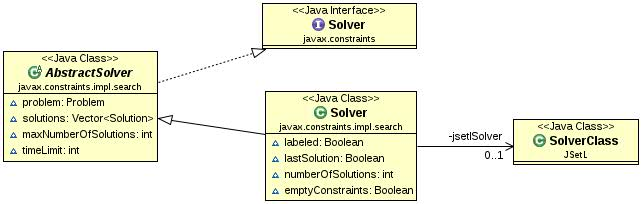
\includegraphics[scale=.5]{img/Solver.JPG}
\caption{Class Diagram di \texttt{Solver}.}
\end{figure}

\subsubsection{Attributi}
La specifica JSR-331, contrariamente a
quanto visto per le variabili ed i vincoli, non prevede che uno specifico
CP solver implementi una classe apposita per un entità solver. Questo 
approccio è ragionevole e non è quindi prevista una struttura come 
\files{CommonBase} in cui sia possibile impostare una implementazione concreta
mediante \files{setImpl}.

Tuttavia JSetL fornisce una classe (\files{SolverClass}) che implementa 
alcune delle proprietà richieste dall'interfaccia \files{Solver}, quindi  viene
utilizzato come attributo \files{private} un'istanza di \files{SolverClass}.
Si elencano di seguito gli attributi aggiunti rispetto alla classe di base:

\begin{lstlisting}[language = Java,
                   caption = {attributi di Solver.}]
	private SolverClass jsetlSolver;
	Boolean lastSolution = false;
	int numberOfSolutions;

	protected JSetL.Constraint[] jsetlConstraints;
	Boolean emptyConstraints = false;
\end{lstlisting}
Come già detto, il primo attributo rappresenta il solver concreto di JSetL.
Segue un attributo booleano: \files{lastSolution} che
indica se nel processo di ricerca si è arrivati all'ultima soluzione valida
per il corrente solver \files{jsetlSolver}. L'attributo
intero rappresentante il corrente numero di soluzioni trovate.

I due attributi separati sono d'ausilio per il passaggio dei vincoli dal
problema a cui il solver è legato al solver JSetL.

\subsubsection{Costruttori}
Vi è un solo costruttore richiesto, che prende come parametro il problema su
cui si costruisce il solver.

\begin{lstlisting}[language = Java,
                   caption = {costruttore di base.}]
public Solver(Problem problem) {
        super(problem);
        jsetlSolver = new SolverClass();
        numberOfSolutions = 0;
        getProblemConstraints();
        setProblemConstraints();
}
\end{lstlisting}
Qui viene chiamato il costruttore della classe astratta di base con il solito
costrutto \files{super(problem)}, quindi viene istanziato l'attributo
\files{jsetlSolver} mediante il suo costruttore. Il numero di soluzioni è
impostato a $0$. Una volta inizializzati i membri propri della classe, mediante
i metodi privati \texttt{getProblemConstraints} e \texttt{setProblemConstraints}
vengono caricati i vincoli presenti nel problema (al momento dell'istanziazione
del solver) e quindi salvati nello \emph{store} JSetL.

\begin{lstlisting}[language = Java,
                   caption = {metodi privati per caricare i vincoli.}]
private void setProblemConstraints() {
        if (emptyConstraints) 
                return;
        for (JSetL.Constraint c : jsetlConstraints)
                jsetlSolver.add(c);
}

private void getProblemConstraints() {
        jsetlConstraints = ((Problem) getProblem()).getJSetLConstraints();
        if (jsetlConstraints == null)
                emptyConstraints  = true;
        else emptyConstraints = false;
}
\end{lstlisting}


\subsubsection{Metodo \texttt{newSearchStrategy}}
\files{newSearchStrategy} è un metodo che consente all'utente di creare una 
nuova strategia di ricerca
per il solver specifico, \files{Solver} in questo caso funziona praticamente 
come una factory.
\begin{lstlisting}[language = Java,
                   caption = {\files{newSearchStrategy}.}]
	public SearchStrategy newSearchStrategy() {
		return new SearchStrategy(this);
	}
\end{lstlisting}
Questo metodo restituisce semplicemente la chiamata ad un costruttore della
classe \files{SearchStrategy}.

\subsubsection{Risoluzione del problema}
Questa parte sella sezione è dedicata alla ricerca delle soluzioni, verranno qui
definiti i metodi \files{findSolution},  \files{findOptimalSolution} e 
\files{findAllSolutions}.

\subsubsection{Metodo \texttt{findSolution}}
Il metodo \files{findSolution} di cui viene richiesta l'implementazione nelle
specifiche è quello con parametro (\files{ProblemState}). Tale parametro
definisce se, dopo la ricerca, lo stato del problema vada ristabilito o meno.

\begin{lstlisting}[language = Java,
                   caption = {\files{findSolution}.}]  
public Solution findSolution(ProblemState restoreOrNot) { 
  applyHeuristic();
  Solution solution = null;
  if(restoreOrNot == ProblemState.RESTORE) {
      .
      .
      .
  } else if(restoreOrNot == ProblemState.DO_NOT_RESTORE) { 
      try { 
        jsetlSolver.solve(); 
        solution = new Solution(this,  
                      numberOfSolutions++); 
      } catch (Failure e) {
          solution = null; 
          e.printStackTrace(); 
        } 
  } 
  return solution;  
}
\end{lstlisting}
Il metodo applica le euristiche sulle variabili del problema con
\files{applyHeuristic}, che verrà discusso in seguito, quindi procede con la
ricerca della soluzione.

A questo punto la computazione ha un punto di scelta, ovvero se lo stato del 
problema va ristabilito al termine della ricerca o meno. 

Il caso \texttt{DO\_NOT\_RESTORE}, più semplice del primo, applica
semplicemente il metodo \files{solve} al solver JSetL, che se troverà una 
soluzione verrà salvata nella variabile \texttt{solution}, altrimenti 
sarà lanciata un'eccezione e catturata subito dopo, impostando a \texttt{null}
la variabile stessa. Il costruttore di 
\files{Solution}, come vedremo nella sezione \ref{jsetlSolution},
salverà ogni variabile del problema internamente.

\begin{lstlisting}[language = Java,
                   caption = {\files{findSolution} il caso \texttt{RESTORE}.}] 
    if(restoreOrNot == ProblemState.RESTORE) {
            if(jsetlSolver.check()) {
                    lastSolution = false;
                    try {
                         solution = new Solution(this, 
                                    numberOfSolutions++);
                    } catch (Failure e) {
                            e.printStackTrace();
                            return null;
                    }
            }
            else return null;
    }
\end{lstlisting}
Il parametro \texttt{RESTORE} è utilizzato principalmente dal metodo
\texttt{hasNext} della classe \texttt{SolutionIterator}. Concettualmente
il suo significato può essere espresso come il ripristino dello stato del 
problema fino all'ultimo punto di scelta, per poter generare quindi la soluzione
successiva. Per implementare questo concetto si è optato per utilizzare la
funzione \texttt{check} del solver JSetL che consente di generare una soluzione
senza svuotare il \texttt{constraint store}.

\subsubsection{Metodo \texttt{findOptimalSolution}}
Come suggerisce il nome, questo metodo ricerca una soluzione ottimale per il
problema. Per fare ciò l'algoritmo dovrebbe esplorare l'intero spazio delle 
soluzioni e memorizzare quella più vicina all'obiettivo. In realtà si è adottato
un sistema per ridurre tale spazio, propagando vincoli sulla
variabile obiettivo, analogamente all'approccio adottato dall'implementazione
comune.
La descrizione del metodo verrà spezzata in più parti, poiché è piuttosto
lungo e composto da più istruzioni correlate.
\begin{lstlisting}[language = Java,
                   caption = {\files{findOptimalSolution}, inizializzazione.}]
public Solution findOptimalSolution(Objective objective, Var objectiveVar) {
	addObjective(objectiveVar);
	long startTime = System.currentTimeMillis();
	if (objectiveVar.getName().isEmpty())
		objectiveVar.setName("Objective"); 
	if (getProblem().getVar(objectiveVar.getName()) == null) {
		getProblem().add(objectiveVar);
	}
	javax.constraints.Var obj = objectiveVar;
	JSetL.Constraint c = new JSetL.Constraint();
	IntLVar target = (IntLVar) obj.getImpl();
	Boolean maximize = false;
	int bestValue = Integer.MAX_VALUE /2;
	if(objective.equals(Objective.MAXIMIZE)) {
		maximize = true;
		bestValue = - Integer.MAX_VALUE /2;
		c.and(target.gt(bestValue));
	} else 	c.and(target.lt(bestValue));
	Solution solution = null;  
\end{lstlisting}
Inizialmente il metodo deve occuparsi di definire l'obiettivo e la variabile
coinvolta. Se la variabile non ha un nome glie ne viene assegnato uno di
default, quindi si verifica che questa appartenga alle
variabili del problema, contrariamente viene aggiunta.

L'obiettivo della funzione può essere di minimizzare o massimizare il valore
della variabile data, a questo propostio viene creato un valore pessimo
\files{bestValue} che rappresenta il minimo o il massimo valore
rappresentabile a seconda del parametro \files{Objective} passato. Il nome
della variabile intera \files{bestValue}
potrebbe essere fuorviante, il valore infatti è quello pessimo per
l'obiettivo ma è considerato l'attuale valore migliore. Ad ogni passo 
se il nuovo valore \files{newValue} è migliore, \files{bestValue} verrà 
sostituito da questo.

A supporto di questo approccio viene utilizzato un vincolo JSetL \texttt{c}
relativo alla variabile obiettivo. Se tale variabile deve essere massimizzata
il valore \texttt{target} deve essere maggiore del miglior valore
attuale, viceversa dovrà essere minore.

\begin{lstlisting}[language = Java,
                   caption = {\files{findOptimalSolution}, il ciclo.}]
while(jsetlSolver.check(c)) {
	if(getMaxNumberOfSolutions() > 0 && 
			numberOfSolutions >= getMaxNumberOfSolutions())
		break;
	if(getTimeLimit() > 0) {
		if (System.currentTimeMillis() - startTime > getTimeLimit())
			break;				
	}
        numberOfSolutions++;
        try {
	    solution = new Solution(this, 
                    numberOfSolutions++);
	} catch (Failure e) {
		e.printStackTrace();
		return null;
	}
        .
        .
        .
\end{lstlisting}
Terminata l'inizializzazione si passa al ciclo per la ricerca vera e propria.
In questa parte del codice si evidenziano le condizioni di ingresso e di uscita 
dal ciclo.

Le istruzioni all'interno del \files{while} continuano fintanto che il vincolo
propagato \texttt{c} nel solver JSetL mediante la funzione \texttt{check}, 
è soddisfacibile. 
Internamente al ciclo si trova quindi una nuova soluzione e viene incrementato
di conseguenza il numero delle soluzioni.

Le possibili condizioni di uscita sono le seguenti:
\begin{enumerate}
\item \texttt{check} ritorna \texttt{false}, ovvero non esistono soluzioni
con l'attuale propagazione del vincolo \texttt{c};
\item è impostato un numero limite di soluzioni ed è stato raggiunto o superato;
\item è impostato un tempo limite ed è stato raggiunto o superato.
\end{enumerate}

\begin{lstlisting}[language = Java,
                   caption = {\files{findOptimalSolution}, verifica obiettivo.}
                  ]  
        int newValue;
        if(maximize) {
                newValue = solution.getMin(obj.getName());
                if(bestValue < newValue)
                        bestValue = newValue;
                c.and(target.gt(bestValue));
        }
        else {	
                newValue = solution.getMax(obj.getName());
                if(bestValue > newValue)
                        bestValue = newValue;
                c.and(target.lt(bestValue));
        }
\end{lstlisting}
Questa è la parte, interna al ciclo, che verifica l'obiettivo ed aggiorna 
l'eventuale soluzione ottima, inoltre aggiorna il vincolo che verrà poi
propagato nella successiva esecuzione della \texttt{check}. Ad ogni passaggio 
viene memorizzato il valore
della corrente soluzione nell'intero \files{newValue}, a seconda che 
l'obiettivo sia massimizzare o minimizzare, se il nuovo valore
è migliore di \files{bestValue}, questo viene sostituito.

Ogni volta viene aggiornato il vincolo relativo alla variabile obiettivo: se
occorre massimizzare il vincolo sarà del tipo $\files{target} > 
\files{newValue}$,
altrimenti del tipo  $\files{target} < \files{newValue}$.
\begin{lstlisting}[language = Java,
                   caption = {\files{findOptimalSolution}, termine.}
                  ]
if (solution != null)
   log("Optimal solution is found. Objective: " +solution.getValue(objectiveVar.getName()));
   return solution;
}
\end{lstlisting}

\subsubsection{Metodo \texttt{findAllSolutions}}
L'ultimo metodo implementato per la ricerca delle soluzioni è inerente alla
ricerca di tutte le possibili soluzioni del problema. Come visto per
\files{findSolution} questo metodo applica prima un'euristica per le
variabili ed i valori, poi si occupa della ricerca.

\begin{lstlisting}[language = Java,
                   caption = {\files{findAllSolutions}, inizializzazione.}
                  ]
public Solution[] findAllSolutions() {
  ArrayList<Solution> array = new ArrayList<Solution>();
  applyHeuristic();
  long startTime = System.currentTimeMillis();
  if(jsetlSolver.check() && (this.getMaxNumberOfSolutions() > 0 || this.getMaxNumberOfSolutions() == -1)) {
    
          .
          .  // Ricerca di tutte le soluzioni.
          .
    
  }
  else return null;
  .
  .
  .
\end{lstlisting}
Inizialmente viene creato un nuovo \files{ArrayList} che conterrà le soluzioni
trovate nel processo di risoluzione. Vengono applicate le euristiche su ogni
variabile del problema e quindi viene inizializzato il timer per il controllo
tempo limite.

A questo punto il metodo è pronto ad iniziare la ricerca, mediante l'istruzione 
\files{if} viene controllato che il problema sia soddisfacibile 
(\files{check}) e il numero
di soluzioni sia coerente con la richiesta. All'interno del ciclo 
è definita la ricerca delle soluzioni.

\begin{lstlisting}[language = Java,
                   caption = {\files{findAllSolutions}, ricerca.}
                  ]
	do { 
	    if (getTimeLimit() > 0) {
		if (System.currentTimeMillis() - startTime > 
		getTimeLimit())
                   break;				
	    }
	    Solution solution;
	    try {
		solution = new Solution(this, 
		numberOfSolutions++);
	    } catch (Failure e) {
	        solution = null;
	        e.printStackTrace();
	    }
	    array.add(solution);
	} while(jsetlSolver.nextSolution() && 
		((this.getMaxNumberOfSolutions() > 
		numberOfSolutions) ||
		this.getMaxNumberOfSolutions() == -1));
\end{lstlisting}
Questa parte di codice, interna al ciclo, genera una soluzione mediante il
solito costruttore quindi l'aggiunge al vettore delle soluzioni. Si entra nel 
ciclo solo se una soluzione è ammissibile.

Le condizioni di uscita del ciclo sono le seguenti:
\begin{enumerate}
\item non esiste una nuova soluzione e quindi l'ultima valida è effettivamente
quella aggiunta nell'array;
\item si è superato il numero di soluzioni massime e quindi l'ultima soluzione
trovata era quella con numero massimo;
\item si è raggiunto o superato il tempo limite.
\end{enumerate}

A questo punto, poiché il metodo richiede che venga restituito un array di 
soluzioni (e non un \files{ArrayList}), questo viene creato e restituito:
\begin{lstlisting}[language = Java,
                   caption = {\files{findAllSolutions}, calcolo del risultato.}
                  ]
  Solution[] result = new Solution[array.size()];
  for (int i = 0; i < result.length; i++) {
    result[i] = array.get(i);
  }
  return result;
}
\end{lstlisting}

\subsubsection{Metodi ausiliari}
Questa parte della sezione è dedicata alle funzioni ausiliarie all'interno
della classe, tra i metodi più rilevanti si evidenziano:
\begin{lstlisting}[language = Java, frame = single]
private void applyHeuristic();
public void addJSetLConstraint(JSetL.Constraint c);
\end{lstlisting}
Ogni metodo sopra elencato è importante perché influenza il solver aggiungendo
vincoli al problema.

\subsubsection{Metodo \texttt{applyHeuristic}}
Questo metodo aggiunge al solver (\files{jsetlSolver}) i vincoli che hanno a che
fare con le euristiche di scelta delle variabili e dei valori che si vogliono
assegnare.
\begin{lstlisting}[language = Java,
                   caption = {\files{applyHeuristic}.}
                  ]
private void applyHeuristic() {
  Vector<javax.constraints.SearchStrategy> strategies = 
      getSearchStrategies();
  if (strategies.isEmpty()) {
    SearchStrategy strategy = (SearchStrategy) getSearchStrategy();
    strategy.label();
    strategy.labelSets();
  }
  else {
       for (int i = 0; i < strategies.size(); i++) {
         SearchStrategy strategy = strategies.elementAt(i);
         ((SearchStrategy) strategy).label();
         ((SearchStrategy) strategy).labelSets();
       }
   }
}
\end{lstlisting}
Il metodo  carica semplicemente le strategie di ricerca in un 
\files{Vector}. Se nessuna strategia è stata precedentemente definita ne
viene creata una di default mediante il metodo \files{getSearchStrategy}, quindi
vengono chiamati i metodi di labeling della classe \files{SearchStrategy}.
Se sono state caricate più di una strategia, per ognuna di esse viene 
effettuato il labeling.

\subsubsection{Metodo \texttt{addJSetLConstraint}}
Il metodo in questione è utilizzato per aggiungere un vincolo JSetL direttamente
al solver \files{jsetlSolver}.
\begin{lstlisting}[language = Java,
                   caption = {\files{addJSetLConstraint}.}
                  ]
public void addJSetLConstraint(JSetL.Constraint c) {
	jsetlSolver.add(c);
}
\end{lstlisting}



\section{Interfaccia \texttt{SearchStrategy}}
La specifica JSR-331 utilizza il concetto di Search Strategy per permettere
ad un utente di scegliere tra differenti algoritmi di ricerca forniti
dalle differenti implementazioni. Le strategie di ricerca sono utilizzate
dai metodi dei solver che si occupano di trovare una soluzione.

Una strategia di ricerca dovrebbe conoscere tutte le variabili di cui si dovrà
assegnare un valore e potrebbero essere necessari
selettori esterni per le variabili ed i valori.

Ogni solver dovrebbe fornire almeno una strategia di ricerca 
 di default da utilizzare nei costruttori del \files{Solver}.

\subsection{Lista d'esecuzione}
La lista d'esecuzione delle strategie di ricerca  consente agli utenti di 
mescolare le strategie per i diversi tipi di variabili e di controllare
l'ordine di assegnamento dei valori. Ad esempio, per la pianificazione e per
problemi di allocazione delle risorse, un utente può decidere prima di 
programmare tutte le attività e poi assegnare le risorse alle attività già 
programmate. Ma  può anche decidere di assegnare prima le risorse e solo 
allora di programmare le attività in base alla disponibilità delle risorse.

\`E stato quindi fornito un sistema per cui l'utente può specificare diverse
strategie per insiemi di variabili differenti. Il metodo della classe
\files{Solver}
\begin{center}
\lstinline[language = Java]$SearchStrategy newSearchStrategy();$
\end{center}
restituisce una nuova istanza per la strategia di default della particolare
implementazione JSR-331 in uso. L'utente può quindi specificare su questa
strategia delle euristiche per le variabili ed i valori e quindi aggiungere la
nuova strategia modificata alla lista d'esecuzione.

Di seguito si mostra un semplice esempio.
\begin{lstlisting}[language = Java,
                   caption = {due differenti strategie.}]
Solver solver = problem.getSolver();
SearchStrategy typeStrategy = solver.getSearchStrategy();
typeStrategy.setVars(types);
SearchStrategy countStrategy = solver.newSearchStrategy();
countStrategy.setVars(counts);
countStrategy.setVarSelectorType(VarSelectorType.MIN_DOMAIN);
solver.addSearchStrategy(countStrategy);
solution = solver.findSolution();
\end{lstlisting}
Sono presenti altri metodi utili per specificare strategie di ricerca senza
dover esplicitamente creare nuove istanze di \files{SearchStrategy}. Il
metodo \files{addSearchStrategy} ad esempio supporta differenti combinazioni di 
parametri \files{Var[]}, \files{VarSelector} e \files{ValueSelector}. Il codice 
di cui sopra può essere riscritto in un modo più conciso:
\begin{lstlisting}[language = Java,
                   frame = single]
Solver solver = problem.getSolver();
solver.getSearchStrategy().setVars(types);
solver.addSearchStrategy(counts, VarSelectorType.MIN_DOMAIN);
solution = solver.findSolution();
\end{lstlisting}

\subsection{Variable Selector}
JSR-331 specifica un insieme di selettori di variabili standard che possono
essere usati dall'utente per personalizzare la strategia. Queste
euristiche sono definite dall'interfaccia standard \files{VariableSelector}
utilizzando il seguente tipo enumerativo:
\begin{lstlisting}[language = Java,
                   frame = single]
static public enum VarSelectorType {
    INPUT_ORDER,
    MIN_VALUE,
    MAX_VALUE,
    MIN_DOMAIN,
    MIN_DOMAIN_MIN_VALUE,
    MIN_DOMAIN_RANDOM,
    RANDOM,
    MIN_DOMAIN_MAX_DEGREE,
    MIN_DOMAIN_OVER_DEGREE,
    MIN_DOMAIN_OVER_WEIGHTED_DEGREE,
    MAX_WEIGHTED_DEGREE,
    MAX_IMPACT,
    MAX_DEGREE,
    MAX_REGRET,
    CUSTOM
}
\end{lstlisting}
Non tutte queste euristiche devono essere fornite da ogni implementazione
concreta di JSR-331.

\subsection{Value Selector}
JSR-331 specifica un insieme di selettori di valori standard che possono
essere usati dall'utente per personalizzare la strategia. Queste
euristiche sono definite dall'interfaccia standard \files{ValueSelector}
utilizzando il seguente tipo enumerativo:
\begin{lstlisting}[language = Java,
                   frame = single]
static public enum ValueSelectorType {
    IN_DOMAIN,
    MIN,
    MAX,
    MIN_MAX_ALTERNATE,
    MIDDLE,
    MEDIAN,
    RANDOM,
    MIN_IMPACT,
    CUSTOM
}
\end{lstlisting}
Non tutte queste euristiche devono essere fornite da ogni implementazione
concreta di JSR-331.

\subsubsection{Euristiche in JSetL}
Prima di passare alla descrizione della classe \files{SearchStrategy} che
fornisce l'implementazione per le strategie di ricerca, occorre sottolineare
che l'approccio alle strategie di selezione delle variabili e dei valori è
differente da quello ipotizzato nella specifica.

La specifica presuppone che le variabili siano selezionate prima, per poi 
essere passate ad un risolutore che vi assegni un valore; infatti 
all'interno del \files{package} 
\files{javax.constraints.impl.search.selectors} fornito dalla specifica
sono definiti vari selettori predefiniti.

JSetL si basa su un sistema molto differente, sfruttando il solver ed 
aggiungendo vincoli di labeling, come già accennato nel capitolo \ref{jsetl} e 
come verrà sottolineato poco più avanti. Per questa ragione, le euristiche di
cui sopra sono state mappate su quelle definite in JSetL per il labeling.

\begin{notabene}
Di contro, questo approccio rende impossibile per l'utente definire una
propria strategia come invece la specifica descritta in \cite{specifiche} 
richiederebbe. 
\end{notabene}

\section{Classe \texttt{SearchStrategy}}\label{search}
La classe \files{SearchStrategy} implementa l'interfaccia standard 
 estendendo la classe \files{AbstractSearchStrategy} 
dell'implementazione comune.
\begin{lstlisting}[language = Java, frame = single]
public class SearchStrategy extends AbstractSearchStrategy {
\end{lstlisting}

Questo approccio permette di ereditare tutti i metodi astratti puri da 
implementare e, dove necessario, ridefinire i metodi non astratti.

\subsection{Classe \texttt{AbstractSearchStrategy}}
La classe astratta \files{AbstractSearchStrategy} estende la classe
\files{CommonBase} descritta nella sezione \ref{common}, poiché come
accennato precedentemente, la specifica si aspetta che ogni implementazione
concreta disponga di una classe che rappresenti la strategia.

JSetL non ha questa caratteristica, tuttavia si è deciso di utilizzare la
classe astratta poiché fornisce molti attributi e metodi utili.

\subsubsection{Attributi}
Gli attributi della classe \files{AbstractSearchStrategy} sono sei:
\begin{lstlisting}[language = Java, frame = single]
	Solver solver;
	protected Var[] vars;
	protected VarReal[] varReals;
//	protected VarSet[] varSets;
	protected VarSelector varSelector;
	protected ValueSelector valueSelector;
	SearchStrategyType type;
\end{lstlisting}
Il primo è il riferimento al solver a cui la strategia è legata.
Seguono quindi gli array delle variabili della strategia, come si può notare
l'array per le variabili insiemistiche è commentato. Durante lo studio della 
specifica si è cambiato approccio
per quanto riguarda le variabili insiemistiche.

Gli attributi \files{varSelector} e \files{valueSelector} specificano
le euristiche della strategia, mentre \files{type} ne definisce il tipo.

\begin{nota}
Per quanto riguarda l'implementazione concreta basata su JSetL due attributi 
verranno ignorati: \files{varReals} e \files{type}. Il primo perché attualmente 
non sono supportate variabili reali, mentre il secondo per la differenza di 
apporccio nell'applicazione delle euristiche, di fatto ogni strategia sarà di 
tipo \files{SearchStrategyType.DEFAULT}.
\end{nota}

\subsubsection{Metodi utili}
I metodi di utilità generica o che non hanno bisogno di un'implementazione
specifica come quella fornita da JSetL, vengono implementati 
direttamente all'interno della classe \texttt{AbstractSearchStrategy}.
Tra quelli più utilizzati si evidenziano:
\begin{itemize}
\item \lstinline[language=Java]$public Solver getSolver();$

Restituisce il solver associato alla strategia di ricerca.
\item \lstinline[language=Java]$public Var[] getVars();$

Restituisce un array di variabili associate alla strategia d'invocazione.
\item \lstinline[language=Java]$public void setVars(Var[] vars);$

Associa un array di variabili alla strategia d'invocazione.
\item \lstinline[language=Java]$public ValueSelector getValueSelector();$

Restituisce l'euristica di selezione del valore da assegnare alle variabili.
\item \lstinline[language=Java]$public VarSelector getVarSelector();$

Restituisce l'euristica di selezione delle variabili.
\item \lstinline[language=Java]$public void setValueSelector(ValueSelector valueSelector);$

Imposta l'euristica di selezione del valore da assegnare alle variabili.
\item \lstinline[language=Java]$public void setVarSelector(VarSelector varSelector);$

Imposta l'euristica di selezione delle variabili.
\end{itemize}

Altri metodi, come ad esempio \files{setVars} sulle variabili insiemistiche,
sono stati omessi poiché non utilizzati dall'implementazione basata su JSetL
oppure perché sovrascritti dalla stessa, e verranno quindi definiti nella
prossima sezione.

\subsection{Implementazione}
Come già sottolineato nel capitolo, JSetL ha un approccio diverso da quello
previsto dalla specifica, l'implementazione quindi non si avvale appieno
delle funzionalità della classe \files{AbstractSearchStrategy} e della
\files{CommonBase}. Inoltre, utilizzando un approccio diverso anche per
l'implementazione delle variabili insiemistiche si è dovuto specializzare
ulteriormente la classe con attributi e metodi.

\begin{figure}[!ht]\label{searchstrategyUML}
\centering
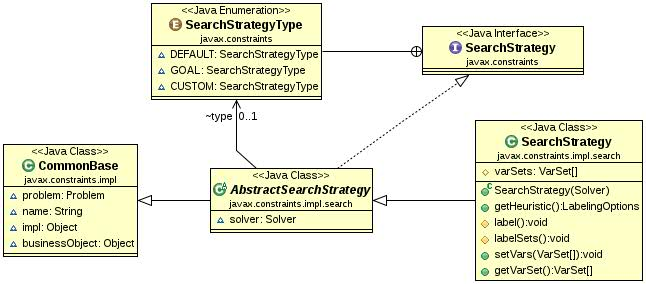
\includegraphics[scale=.5]{img/SearchStrategy.JPG}
\caption{Class Diagram di \texttt{SearchStrategy}.}
\end{figure}

\subsubsection{Attributi}
Poiché nel problema (nella classe \files{Problem}) è stato aggiunto 
un array di variabili insiemistiche legate al problema, anche nella classe 
\files{SearchStrategy}
è stato aggiunto tale array.
\begin{lstlisting}[language = Java, frame = single]
    protected VarSet[] varSets;
\end{lstlisting}
L'attributo \files{varSets} rappresenta le variabili insiemistiche associate 
alla strategia.

\subsubsection{Costruttori}
Vi è un solo costruttore di classe, che prende come unico argomento il
solver a cui è associato:
\begin{lstlisting}[language = Java, frame = single]
public SearchStrategy(Solver solver) {
	super(solver);
	varSets = ((Problem) getProblem()).getSetVars();
}
\end{lstlisting}
Questo chiama il costruttore della classe base, quindi inizializza i due
array mediante la funzione \files{getProblem} che restituisce il problema a 
cui la strategia è associata e quindi da questo ottiene le variabili con
il relativo metodo \files{getSetVars}.

\subsubsection{Euristiche}
In questa parte della sezione verranno specificati i metodi che codificano
ed applicano le euristiche di scelta per assegnare valori alle variabili
e per scegliere l'ordine di assegnamento delle stesse.

\subsubsection{Metodo \texttt{getHeuristic}}
Questa funzione è una vera e propria mappa per le euristiche, ovvero associa
ogni \files{VarSelector} o \files{ValueSelector} della specifica ad
un'euristica di JSetL. La funzione è divisa in due parti, la prima si occupa
delle variabili, la seconda dei valori.
\begin{lstlisting}[language = Java,
                   caption = {\files{getHeuristic}, le variabili.}]
public LabelingOptions getHeuristic() {
	LabelingOptions lop = new LabelingOptions();
	VarSelector varSelector = getVarSelector();
	if (varSelector != null) {
		VarSelectorType varType = varSelector.getType();
		switch(varType) {
		case INPUT_ORDER: 
			lop.var = VarHeuristic.LEFT_MOST;
			break;
		case MIN_VALUE:
			lop.var = VarHeuristic.MIN;
			break;
		case MAX_VALUE:
			lop.var = VarHeuristic.MAX;
			break;
		case RANDOM:
			lop.var = VarHeuristic.RANDOM;
			break;
		case MIN_DOMAIN:
			lop.var = VarHeuristic.FIRST_FAIL;
			break;
		default:
			lop.var = VarHeuristic.LEFT_MOST;
			break;
		}
	}
	else lop.var = VarHeuristic.LEFT_MOST;
\end{lstlisting}
Innazitutto viene inizializzata un'istanza della classe
\files{LabelingOptions}, questa è una classe di supporto JSetL utile per 
definire vincoli di labeling sulle variabili, ovvero le euristiche.

Quindi, mediante il metodo della classe base \files{getVarSelector}, viene
memorizzato il selettore per le variabili. Con lo \files{switch} infine, a 
seconda del caso viene impostato il valore di \files{lop.var} opportuno.
Se nessuno dei casi combacia con quelli identificati viene imposto di default
un'euristica di tipo leftmost, come richiesto dalla specifica.
\begin{lstlisting}[language = Java,
                   caption = {\files{getHeuristic}, i valori.}]
    ValueSelector valueSelector = getValueSelector();
    if (valueSelector != null) {
	ValueSelectorType valueType = valueSelector.getType();
        switch(valueType) {
	case MIN:
		lop.val = ValHeuristic.GLB;
		break;
	case MAX:
		lop.val = ValHeuristic.LUB;
		break;
	case MIDDLE:
		lop.val = ValHeuristic.MID_MOST;
		break;
	case MEDIAN:
		lop.val = ValHeuristic.MEDIAN;
		break;
	case RANDOM:
		lop.val = ValHeuristic.EQUI_RANDOM;
		break;
	default:
		lop.val = ValHeuristic.GLB;
		break;
	}
	return lop;
\end{lstlisting}
Nella parte finale dell'algoritmo si compiono gli stessi passaggi, ma per
la scelta dei valori. Quindi viene restituito il \files{LabelingOptions}
ottenuto.

\subsubsection{Metodo \texttt{label}}
Il metodo \files{label} è il primo metodo implementato e descritto che si
occupa di applicare un'euristica. Questo opera sulle variabili intere della 
strategia.
\begin{lstlisting}[language = Java,
                   caption = {\files{label()}.}]
protected void label() {
	if (vars == null || vars.length == 0)
		return;
	SolverClass sc = ((Solver) getSolver()).getSolverClass();
	IntLVar[] vec = new IntLVar[vars.length];
	for (int i = 0; i < vars.length; i++) {
		vec[i] = (IntLVar) vars[i].getImpl();
	}
	sc.add(IntLVar.label(vec, getHeuristic()));
}
\end{lstlisting}
Dopo aver controllato che il vettore delle variabili intere non sia nullo
(contrariamente il metodo viene interrotto senza errori) viene memorizzato
un riferimento al solver JSetL e viene inizializzato un vettore di
\files{IntLVar} con le implementazioni concrete delle variabili intere
della strategia.

A questo punto viene caricata la strategia mendiante il metodo
\files{getHeuristic} vista sopra, ed aggiunto al solver JSetL un vincolo
speciale di labeling creato mediante la funzione
\files{label(IntLVar[], LabelingOptions)} definita in \cite{tesiAmadini} e di 
cui si
è accennato nel capito \ref{jsetl}.

\subsubsection{Metdo \texttt{labelSets}}
\files{labelSets} si comporta come il metodo per le variabili intere, cambiano
solo i tipi, tecnica e metodi sono i medesimi, si da la definizione per 
completezza.
\begin{lstlisting}[language = Java,
                   caption = {\files{labelSets()}.}]
protected void labelSets() {
	if (varSets == null || varSets.length == 0)
		return;
	SolverClass sc = ((Solver) getSolver()).getSolverClass();
	SetLVar[] vec = new SetLVar[varSets.length];
	for (int k = 0; k < vars.length; k++) {
		vec[k] = (SetLVar) varSets[k].getImpl();
	}
	sc.add(SetLVar.label(vec, getHeuristic()));
}
\end{lstlisting}

\section{Interfaccia \texttt{Solution}}
L'interfaccia standard \files{Solution} specifica le soluzioni che possono
essere generate dai metodi della classe \files{Solver} e dagli iteratori.
Questa interfaccia è completamente implementata nella common implementation
definita dalla classe \files{BasicSolution},
ogni implementazione concreta può estenderla mediante la sottoclasse
\files{Solution}.

Un'istanza della soluzione contiene le copie di tutte le variabili
legate al problema che sono state usate da una strategia di ricerca che ha
creato tale soluzione.

\subsubsection{Metodi}
I metodi e le funzioni definiti nell'interfaccia sono i seguenti:
\begin{itemize}
\item[-]\lstinline[language = Java]$public Var[] getVars();$

Restituisce le variabili della soluzione legate al problema.
\item[-]\lstinline[language = Java]$public Var getVar(String name);$

Restituisce la variabile con il nome dato dalla stringa \files{name}. 
Lancia un'eccezione se la variabile non esiste.
\item[-]\lstinline[language = Java]$public int getValue(String name);$

Restituisce il valore della variabile con il nome dato dalla stringa 
\files{name}. 
Lancia un'eccezione se la variabile non esiste.
\item[-]\lstinline[language = Java]$public boolean isBound();$

Restituisce \files{true} se ogni variabile della soluzione è bound (ovvero
il suo dominio è un singolo valore), \files{false} altrimenti.
\item[-]\lstinline[language = Java]$public boolean isBound(String name);$

Restituisce \files{true} se la variabile con il nome dato  è ``bound'',
\files{false} altrimenti.
\item[-]\lstinline[language = Java]$public int getSolutionNumber();$

Restituisce il numero associato alla soluzione.
\item[-]\lstinline[language = Java]$public void setSolutionNumber(int number);$

Assegna un valore intero al numero associato alla soluzione.
\item[-]\lstinline[language = Java]$public void log();$

Questo metodo stampa la soluzione, è una variante della medesima definita
nell'interfaccia \files{Problem}.
\item[-]\lstinline[language = Java]$public Solver getSolver();$

Restituisce il solver associato alla soluzione.
\end{itemize}

\section{Classe \texttt{Solution}}\label{jsetlSolution}
La classe \files{Solution} implementa l'interfaccia standard
\files{Solution} estendendo la classe \files{BasicSoltion} dell'implementazione
comune.
\begin{lstlisting}[language = Java,
                   frame = single]
public class Solution extends BasicSolution {
\end{lstlisting}
Questo approccio permette di ereditare tutti i metodi della classe base, che
non è astratta, ma una vera e propria implementazione di base
della soluzione. Verrà quindi brevemente descritta.

\subsection{Classe \texttt{BasicSolution}}
\files{BasicSolution} rappresenta l'implementazione di base della soluzione
di un problema, viene fornita nella specifica dal file 
\files{BasicSolution.java} contenuto nel package 
\files{javax.constraints.impl.search}. \`E una classe base, non
estende quindi nessun'altra classe
\begin{lstlisting}[language = Java,
                   frame = single]
public class BasicSolution implements Solution {
\end{lstlisting}

Questa classe implementa totalmente quanto specificato nell'interfaccia, 
pertanto non vi sarebbe il bisogno di specializzarla. Tuttavia poiché nella
implementazione basata su JSetL sono stati introdotti alcuni aspetti che
si discostano dalle specifiche individuate dallo standard, si è dovuto trattare
in modo specializzato quest'ultimi.

\subsubsection{Attributi}
Gli attributi della classe base sono i seguenti:
\begin{lstlisting}[language = Java,
                   frame = single]
	Solver 	        solver;
	int 		solutionNumber;
	ResultInt[] 	intResults;
	ResultReal[] 	realResults;
	ResultSet[] 	setResults;
\end{lstlisting}
\files{solver} rappresenta, come di consueto, il solver da cui la soluzione
è stata generata. L'intero \files{solutionNumber} ne rappresenta il numero
progressivo.

Gli utlimi tre attributi meritano un discorso più dettagliato, questi infatti 
sono degli array di un tipo definito nello stesso file della classe
\files{BasicSolution} e di fatto rappresentano internamente il risultato.

\subsubsection{Classe \texttt{ResultInt}}
\files{ResultInt} rappresenta una delle variabili intere risolta dal solver.
\begin{lstlisting}[language = Java,
                   frame = single]
class ResultInt {
	String varName;
	int value;
	inte min;
	int max;
	boolean bound;
}
\end{lstlisting}
Ha alcuni attributi che ne rappresentano il nome, il valore attuale (se 
unico), il valore minimo e quello massimo, quindi un booleano che indica 
se la variabile risolta è bound, ovvero ha un unico valore possibile. 
Viene fornita anche una funzione \files{toString}.

\subsubsection{Classe \texttt{ResultReal}}
Questa classe è praticamente identica a quella definita per le variabili
intere (cambiano ovviamente i tipi) e, poiché JSetL non supporta i vincoli
sui reali, verrà omessa la descrizione.

\subsubsection{Classe \texttt{ResultSet}}
Anche in questo caso verrà omessa la descrizione della classe, poiché
l'approccio adottato dallo standard è molto differente dall'implementazione
concreta che JSetL fornisce per gli insiemi. Tuttavia a differenza della
struttura sui reali, questa verrà ridefinita nel file della classe
\files{Solution}.

\subsubsection{Metodi}
Si evidenziano alcuni metodi non presenti tra quelli già menzionati 
nelle interfacce che manipolano le sopracitate classi di risultati:
\begin{itemize}
\item[-]\lstinline[language = Java]$private int getIndexOfInt(String name);$

Restituisce l'indice della variabile risolta di nome \files{name}. In caso
la variabile non esista lancia un'eccezione.
\item[-]\lstinline[language = Java]$ResultInt createResult(Var var);$

Questa importante funzione, presa una variabile intera (risolta dal solver),
genera e restituisce un istanza della classe \files{ResultInt}.
\end{itemize}

Al momento della realizzazione dell'implementazione concreta 
lo standard non fornisce il supporto alle variabili reali ed 
insiemistiche. Ovvero nel costruttore di \files{BasicSolution} non è ancora 
implementato l'algoritmo
per generare variabili risolte di tipo \files{ResultReal} e \files{ResultSet}.
Analogamente non è stata introdotta la funzione \files{createResult} per
le suddette variabili. Come si vedrà nella prossima sezione questi meccanismi
per le variabili insiemistiche sono state aggiunte nella specializzazione
\files{Solution}.

\begin{figure}[!ht]\label{solutionUML}
\centering
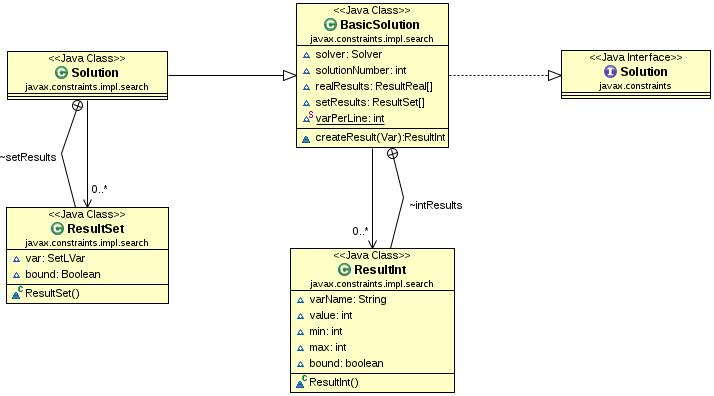
\includegraphics[scale=.5]{img/Solution.JPG}
\caption{Class Diagram di \texttt{Solution}.}
\end{figure}

\subsection{Implementazione}
La parte implementativa dell'interfaccia \files{Solution} verte esclusivamente
sul supporto delle variabili insiemistiche. Per raggiungere tale obiettivo si
è ridefinita la classe \files{ResultSet}, si è aggiunto un attributo come nella
classe base, si è definita la funzione \files{createResult} per variabili
insimistiche e si è specializzato il costruttore.


\subsubsection{Attributi}
L'unico attributo di classe è \files{setResults}, un array di tipo 
\files{ResultSet}. Questo attributo si è dovuto aggiungere causa l'impossibilità
di accedere alla controparte della classe base. Come questa, conterrà
un array di variabili risolte di tipo insiemistico.

\subsubsection{Classe \texttt{ResultSet}}
Come anticipato nella sezione precedente, la classe ausiliaria \files{ResultSet}
è stata ridefinita nel seguente modo:
\begin{lstlisting}[language = Java,
                   caption = {\files{ResultSet}.}]
class ResultSet {
	SetLVar var;
	Boolean bound;
	
	public String toString() {
		return var.toString();
	}
	
	public String getName() {
		return var.getName();
	}
}
\end{lstlisting}
Questa classe è stata creata sul modello di quelle implementate nel file 
dell'implementazione comune
\files{BasicSolution}, ma sfrutta la classe \files{SetLVar}.

\subsubsection{Metodo \texttt{createResult}}
Anche la funzione \files{createResult} è stata implementata seguendo l'approccio
di quella per variabili intere nella classe base.
\begin{lstlisting}[language = Java,
                 caption = {\files{createResult} per variabili insiemistiche.}]
private ResultSet createResult(VarSet var) {
        ResultSet result = new ResultSet();
        if(var.isBound())
                result.bound = true;
        else result.bound = false;
        result.var = (SetLVar) ((VarSet) var).getImpl();
        return result;
\end{lstlisting}
Data una variabile insiemistica \files{var}, questo metodo crea una nuova
istanza della classe \files{ResultSet} e quindi ne assegna i valori.
Se la data variabile è bound l'attributo \files{bound} della
nuova variabile risolta viene impostato a \files{true}, altrimenti a
\files{false}. Quindi nel campo \files{var} viene copiata 
l'implementazione concreta relativa alle variabili insimistiche.

\subsubsection{Costruttore}
La parte più delicata dell'implementazione è il costruttore. 
La descrizione di questo è stata
lasciata per ultima poiché sfrutta il tipo ed il metodo definiti sopra.
\begin{lstlisting}[language = Java,
                 caption = {\files{createResult} per variabili insiemistiche.}]
public Solution(Solver solver, int solutionNumber) throws Failure {
	super(solver, solutionNumber);
	Vector<javax.constraints.SearchStrategy> searchStrategies = 
            ((AbstractSolver)solver).getSearchStrategies();
	Vector<VarSet> strategyVars = new Vector<VarSet>();
	for (javax.constraints.SearchStrategy strategy : searchStrategies) {
		VarSet[] vars = ((SearchStrategy) strategy).getVarSet();
		if (vars == null)
			return;
		for (VarSet var : vars) {
			if (!strategyVars.contains(var))
				strategyVars.add(var);
		}
	}
	setResults = new ResultSet[strategyVars.size()];
	Iterator<VarSet> iter = strategyVars.iterator();
	int i = 0;
	while(iter.hasNext()) {
		VarSet var = iter.next();
		setResults[i++] = createResult(var);
	}	
}
\end{lstlisting}
Analogamente a quanto visto finora si è seguito l'approccio dell'implementazione
di base. Brevemente, il costruttore chiama quello della classe base, quindi
applica gli stessi costrutti per creare le variabili risolte ed inserirle 
nell'array dei risultati (specializzato).

Si evidenziano due fasi: nella prima vengono caricate tutte le strategie e 
per ogni strategia si salvano le variabili insimistiche coinvolte; nella
seconda fase viene creato l'array dei risultati che viene poi riempito
tramite la funzione \files{createResult}.


\section{Interfaccia \texttt{SolutionIterator}}
L'interfaccia standard \files{SolutionIterator} consente all'utente di trovare
e navigare tra diverse soluzioni ed eseguire differenti azioni specifiche
sulle soluzioni trovate.

L'utilizzo, come si intende nella specifica, è presentato in questo esempio:
\begin{lstlisting}[language = Java,frame = single]
SolutionIterator iter = solver.solutionIterator();
while(iter.hasNext()) {
  Solution solution = iter.next();
  ...
}
\end{lstlisting}

I metodi previsti dall'interfaccia sono solo due: \files{hasNext} che controlla
se c'è una nuova soluzione e \files{next} che genera la nuova soluzione.

\subsection{Classe \texttt{BasicSolutionIterator}}
L'implementazione comune fornisce una classe di base che implementa
l'interfaccia \files{SolutionIterator}. Questa non è stata presa in 
considerazione per
l'implementazione concreta JSetL e non verrà quindi descritta.

\section{Classe \texttt{SolutionIterator}}\label{solIter}
La classe \files{SolutionIterator} implementa l'interfaccia
\files{SolutionIterator} direttamente, senza appoggiarsi a classi di base.
\begin{lstlisting}[language = Java,frame = single]
public class SolutionIterator implements javax.constraints.SolutionIterator {
\end{lstlisting}


\subsubsection{Attributi}
Si definiscono i seguenti attributi:
\begin{lstlisting}[language = Java,frame = single]
	Solver solver;
	int solutionNumber;
	Boolean hasNext;
	Boolean checked = false;
        private boolean firstcall = true;
\end{lstlisting}
Come di consueto per le classi che rappresentano la soluzione, il primo 
attributo è il \files{solver} legato alla soluzione, quindi segue il numero
identificativo della stessa. \files{hasNext} è un valore booleano che
specifica se è presente una nuova soluzione, \files{checked} invece
è utilizzato per verificare che la funzione \files{hasNext} sia stata
invocata prima della funzione \files{next}. L'ultimo attributo verifica
che la funzione \texttt{hasNext} sia o meno invocata la prima volta.

\subsubsection{Costruttore}
L'unico costruttore richiesto è quello con parametro di tipo \files{Solver}:
\begin{lstlisting}[language = Java,
                   caption = {il costruttore di \files{SolutionIterator}.}]
public SolutionIterator(Solver s) {
	solver = (Solver) s;
	hasNext = true;
	solutionNumber = 0;
}
\end{lstlisting}
Questo imposta l'attributo \files{solver} con il solver che ha generato la
soluzione, imposta di default l'attributo \files{hasNext} a \files{true}
ed il numero di soluzione a $0$.

\subsubsection{Metodo \texttt{hasNext}}
Il metodo \files{hasNext} controlla che esista una soluzione successiva
all'interno dello stato del solver. Per fare ciò cerca una soluzione con il
metodo \files{findSolution} con parametro \files{ProblemState.RESTORE}, in
modo tale da permettere al solver di mantenere i punti di scelta ed iterare il
procedimento.
\begin{lstlisting}[language = Java,
                   caption = \files{hasNext}.]
public boolean hasNext() {
        checked = true;
        if (firstcall) {
                firstcall = false;
                Solution solution = solver.findSolution(ProblemState.RESTORE);
                if (solution == null) {
                        hasNext = false;
                        return false;
                }
                return true;
        }
        return solver.hasNext();
\end{lstlisting}
Inizialmente imposta \files{checked} al valore \files{true}, quindi se è 
la prima chiamata \texttt{firstcall} viene impostata a \texttt{true} quindi
cerca la soluzione.
Se la soluzione trovata non è nulla restituisce \files{true}, altrimenti
imposta l'attributo \files{hasNext} a \files{false} e restituisce
\files{false}.

Nel caso in cui la chiamata al metodo non è la prima, il risultato viene
demandato all'omonima funzione della classe \texttt{Solver} che semplicemente
sfrutta la funzione \texttt{nextSolution} del solver JSetL.


\begin{notabene}
\`E importante sottolineare che l'unico caso in cui viene usata la funzione
\files{findSolution} con il parametro \files{ProblemState.RESTORE}
all'interno dell'implementazione comune è nel relativo metodo \files{hasNext}
della classe \files{BasicSolutionIterator}.
Questo perché, secondo l'approccio utilizzato nella specifica JSR-331, 
\files{ProblemState} modella il controllo per il \emph{Backtracking}.

In JSetL il backtracking è insito nel solver e, per sfruttarlo, si utilizza la 
funzione
\files{nextSolution}, senza bisogno di un punto di
scelta. Per questo motivo, nella classe \files{Solver} il metodo
\files{findSolution} utilizza \files{nextSolution} nel
caso il parametro passato sia \files{RESTORE}.
\end{notabene}

\begin{figure}[!ht]\label{solutioniteratorUML}
\centering
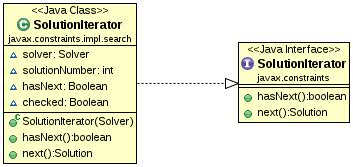
\includegraphics[scale=.75]{img/SolutionIterator.JPG}
\caption{Class Diagram di \texttt{SolutionIterator}.}
\end{figure}

\subsubsection{Metodo \texttt{next}}
Questo metodo crea la soluzione trovata dal metodo \files{hasNext} e la
restituisce. \`E quindi necessario che ogni volta che questo viene chiamato
sia stato precedentemente invocato \files{hasNext}. A questo proposito
viene sfruttato l'attributo \files{checked}: inizialmente il medoto controlla
che questo sia \files{true} (ovvero \files{hasNext} è stato utilizzato),
quindi prima dell'uscita lo reimposta a \files{false}, in modo tale che
\files{hasNext} debba essere richiamato nuovamente in seguito.

\begin{lstlisting}[language = Java,
                   caption = \files{next}.]
public Solution next() {
	if (!checked)
		throw new RuntimeException("Cannot use SolutionIterator.next() " + "before checking the hasNext() returned true");
	Solution solution;
	try {
		solution = new Solution(solver, solutionNumber);
		solution.setSolutionNumber(solutionNumber);
		solutionNumber++;
	} catch (Failure e) {
		e.printStackTrace();
		hasNext = false;
		return null;
	}
	checked = false;
	return solution;
}
\end{lstlisting}
All'interno del metodo viene creata la soluzione mediante il costruttore
fornito dalla classe \files{Solution} che automaticamente genera
le variabili risolte. Viene quindi aggiornato il numero di soluzione.


